
Методы решения задач компьютерного зрения включают как классические подходы, так и глубокие нейронные сети.

Классические методы основываются на внутренней структуре и симметрии изображения, 
его семантике и характеристиках объектов на нем. 
Эти методы включают в себя алгоритмы обработки изображений,
 фильтрацию, выделение признаков (например, метод гистограмм градиентов или методы локтевых точек),
  шаблонное сопоставление и классификацию на основе характеристик объектов.

\texit{Определение}\textbf{Сверточные нейронные сети} (CNN)\cite{lecun1989handwritten} представляют собой класс глубоких нейронных сетей,
использующих
специально разработанных для обработки структурно связанных данных как изображения. 
Эффективность сетей связывают с их способностью автоматически извлекать иерархические признаки из входных данных.

Глубокие методы, основанные на сверточных нейронных сетях (CNN), 
стали широко распространенными и эффективными в решении задач компьютерного зрения. 
Эти методы автоматически изучают признаки изображений на различных уровнях абстракции, 
начиная от низкоуровневых признаков, таких как грани и текстуры, до высокоуровневых семантических признаков,
 связанных с объектами и их распознаванием. 
 
Основой глубоких сверточных сетей являются

\begin{figure}[h]
    \centering
    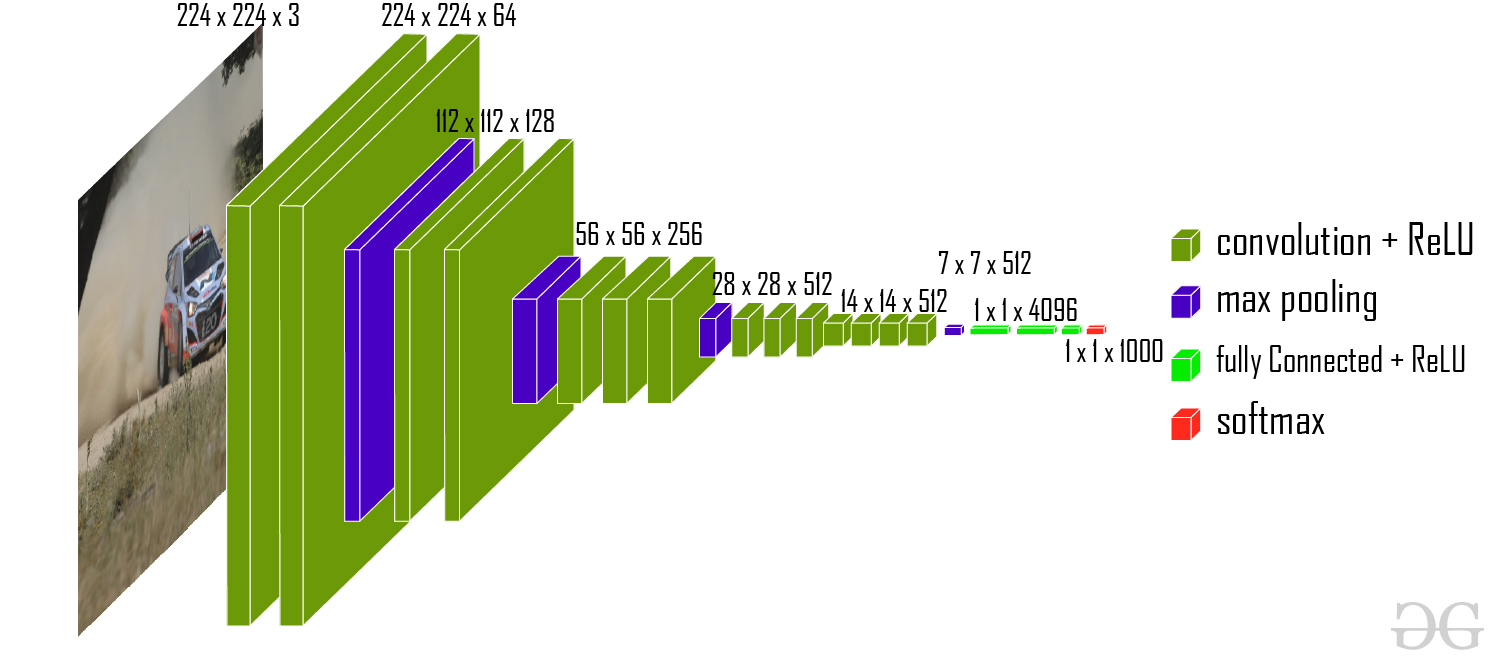
\includegraphics[width=0.5\textwidth]{assets/ml/cv/vgg16.jpg}
    \caption{Архитектура VGG16 \cite{simonyan2014very}}
    \label{vgg_arch}
\end{figure}

Cверточные, пулинговые и полносвязные слои, которые работают в совокупности для изучения и классификации изображений.

Эти два класса методов часто комбинируются для достижения лучших результатов в решении задач компьютерного зрения. Например, глубокие нейронные сети могут использоваться для извлечения признаков из изображений, а затем классические методы могут применяться для анализа этих признаков и решения конкретных задач, таких как детекция объектов или сегментация изображений.


Основными компонентами сверточных нейронных сетей являются \begin{itemize}
    \item сверточные слои
    \item пулинг слои
    \item полносвязанные слои.
\end{itemize}

\textit{Определение} \textbf{Cверточные} слои выполняют операции свертки над входными данными с использованием фильтров или ядер, 
чтобы извлечь локальные пространственные признаки, такие как грани, углы и текстуры. Это позволяет модели обнаруживать абстрактные особенности изображений на разных уровнях детализации.

\textit{Определение} \textbf{Пулинг} слои предназначены для уменьшения пространственных размеров активаций, полученных после сверточных операций, путем объединения значений пикселей в заданных областях. Это позволяет модели быть инвариантной к небольшим трансляциям объектов на изображении и уменьшает количество параметров, что способствует предотвращению переобучения и повышению эффективности вычислений.



Полносвязанные слои обычно располагаются в конце архитектуры нейронной сети и используются для объединения высокоуровневых признаков, извлеченных предыдущими слоями, в предсказания или классификации. Эти слои обладают полным соединением со всеми активациями предыдущего слоя и представляют собой типичные слои нейронных сетей, в которых каждый нейрон связан с каждым нейроном предыдущего слоя.

Во время обучения сверточной нейронной сети параметры каждого слоя оптимизируются с использованием методов оптимизации, таких как обратное распространение ошибки и стохастический градиентный спуск, с целью минимизации заданной функции потерь. Этот процесс позволяет модели настраивать свои параметры для эффективного извлечения признаков и выполнения конкретной задачи, такой как классификация изображений или сегментация объектов.


\begin{figure}[h]
    \centering
    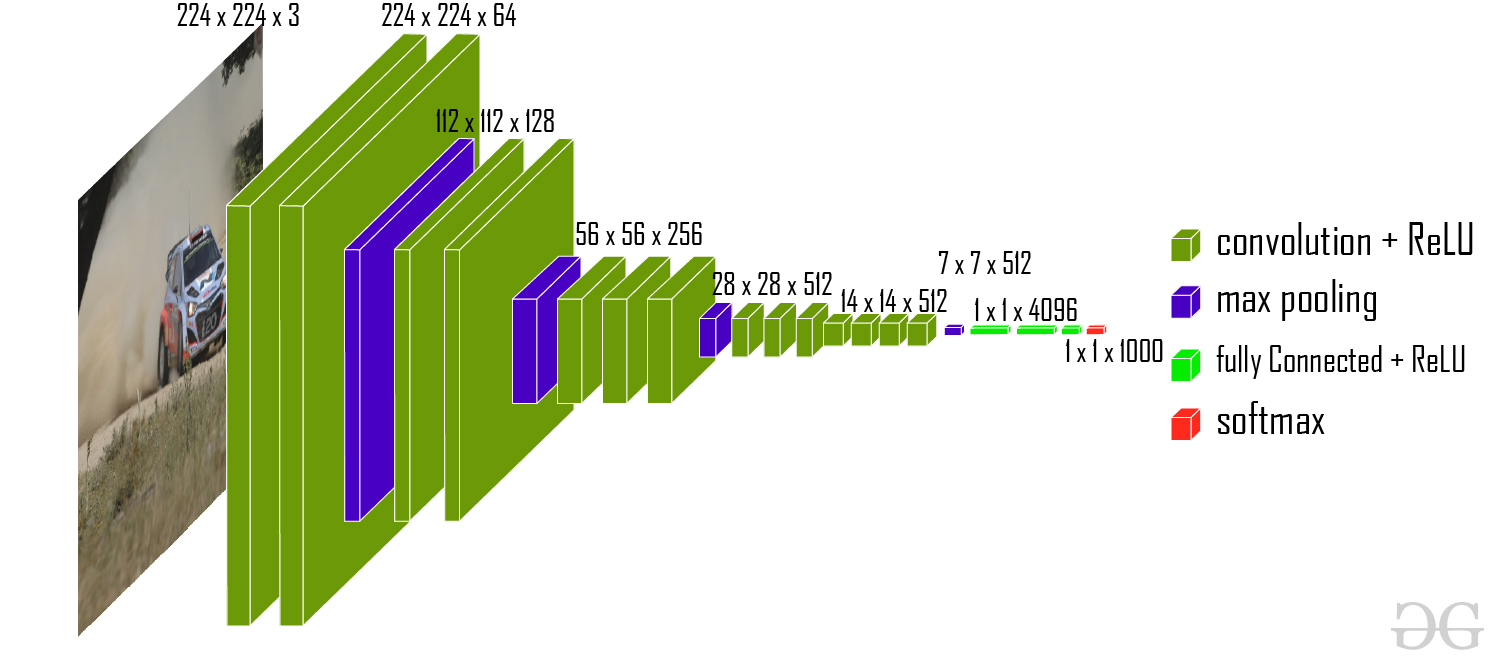
\includegraphics[width=0.5\textwidth]{assets/ml/cv/vgg16.jpg}
    \caption{Архитектура VGG16 \cite{simonyan2014very}}
    \label{vgg_arch}
\end{figure}


Архитектуры U-Net \ref{unet_arch}  и ResNet \ref{vgg_arch} являются двумя широко используемыми моделями в области компьютерного зрения, обе из которых имеют уникальные характеристики и применяются в различных задачах.

U-Net - это архитектура, разработанная для сегментации изображений, особенно в медицинском изображении. Ее особенностью является использование симметричной структуры, включающей свертки (downsampling) для уменьшения размерности и деконволюционные слои (upsampling) для восстановления пространственного разрешения. Основное преимущество U-Net заключается в способности эффективно обрабатывать маленькие объекты и сохранять детали на всех уровнях.

\begin{figure}[h]
    \centering
    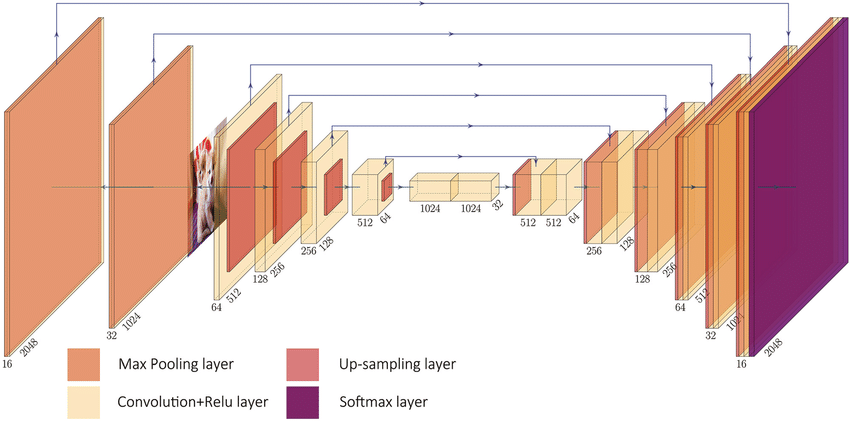
\includegraphics[width=0.5\textwidth]{assets/ml/cv/unet.png}
    \caption{Архитектура Unet \cite{ronneberger2015u}}
    \label{unet_arch}
\end{figure}

Основные параметры конволюции \begin{itemize}
    \

\end{itemize}


ResNet, с другой стороны, известен своей глубокой архитектурой с использованием блоков с пропуском (skip connections), которые обеспечивают плавное обучение глубоких сетей. Основное преимущество ResNet заключается в способности обучать глубокие модели с минимальным ухудшением производительности (проблема затухающих градиентов), благодаря использованию пропускающих соединений.



Методы аугментации изображений в компьютерном зрении представляют собой техники, используемые для увеличения размера и разнообразия тренировочного набора данных путем применения различных преобразований к изображениям. 
Целью аугментации является создание дополнительных вариаций изображений, что помогает улучшить обобщающую способность моделей машинного обучения и уменьшить риск переобучения.

Основные методы аугментации включают в себя
\begin{itemize}
    \item изменение размера изображения (путем масштабирования)
    \item  повороты и отражения 
    \item  изменение яркости, контраста и насыщенности цвето
    \item добавление шума или размытия.
\end{itemize}    
    
Дополнительно, могут применяться специфические трансформации, такие как сдвиги, обрезки или изменение геометрии изображения.

Применение методов аугментации позволяет модели машинного обучения обучаться на более разнообразных данных, 
что способствует повышению их устойчивости к различным условиям и изменениям в данных во время работы.
Кроме того, аугментация может помочь справиться с проблемой несбалансированных классов и улучшить обобщающую способность моделей.


Модель YOLO (You Only Look Once) представляет собой популярную архитектуру для обнаружения объектов на изображениях. Ее основной идеей является выполнение обнаружения объектов и классификации в одной сети, что делает ее быстрой и эффективной.
\cite{kirillov2023segment}
Порядок работы модели YOLO начинается с входного изображения, которое подается на вход нейронной сети. Затем изображение проходит через сверточные слои, которые извлекают признаки из изображения на различных уровнях абстракции.

Далее, полученные признаки пропускаются через сверточные слои, которые прогнозируют боксы (ограничивающие рамки) для объектов и их вероятности принадлежности к различным классам. Эти сверточные слои производят прогнозы на основе якорей (anchors), которые представляют разные размеры и соотношения сторон боксов.

После этого выполняется пост-обработка, включающая подавление неоднородных предсказаний (non-maximum suppression), чтобы получить финальные прогнозы объектов. Этот шаг удаляет лишние дубликаты и уверенно прогнозирует объекты с наибольшей уверенностью (confidence).

В результате работы модели YOLO получается набор боксов с классами и оценками уверенности, представляющих объекты, найденные на изображении. Эта информация может быть использована для обнаружения объектов и их классификации в реальном времени.

\subsubsection{Выделение объектов}


Алгоритм bounding box представляет собой метод в области компьютерного зрения, направленный на выделение прямоугольной области, охватывающей объекты на изображении. Основная цель алгоритма состоит в определении минимального прямоугольника, который содержит объект, сохраняя при этом минимальные потери информации.

Принцип работы алгоритма bounding box заключается в следующих шагах:

1. Подготовка изображения: Изображение предварительно обрабатывается для улучшения качества и подготовки к дальнейшему анализу.
2. Обнаружение объектов: Проводится анализ изображения с целью выявления интересующих областей, используя различные методы, такие как выделение краев, сегментация или классификация.
3. Вычисление ограничивающих рамок: Для каждого обнаруженного объекта определяется минимальный прямоугольник, который полностью охватывает его.
4. Визуализация результатов: Ограничивающие рамки визуализируются на изображении для дальнейшего анализа или использования.

Математически алгоритм bounding box может быть описан следующим образом:

Пусть \( P = \{p_1, p_2, ..., p_n\} \) — множество точек, описывающих объект на изображении.

Координаты верхнего левого угла ограничивающей рамки $(x_{min}, y_{min})$ и координаты нижнего правого угла $(x_{max}, y_{max})$ определяются как:

\[ x_{\text{min}} = \min_{p \in P} (p_x), \]
\[ y_{\text{min}} = \min_{p \in P} (p_y), \]
\[ x_{\text{max}} = \max_{p \in P} (p_x), \]
\[ y_{\text{max}} = \max_{p \in P} (p_y). \]

Таким образом, алгоритм bounding box позволяет эффективно выделять и описывать объекты на изображении, что является важным инструментом в области компьютерного зрения и обработки изображений.


Процедура разметки в области компьютерного зрения (computer vision) представляет собой процесс создания аннотаций или меток для изображений с целью обучения моделей машинного обучения. Этот процесс включает в себя несколько шагов и может быть выполнен как вручную, так и с использованием специализированных инструментов.

Один из основных методов разметки вручную - это создание прямоугольных или многоугольных областей (bounding boxes) вокруг объектов интереса на изображении. Эти bounding boxes обозначают положение и размер объекта на изображении. Для каждого bounding box также указывается класс объекта (например, кошка, собака, машина и т. д.).

Другой метод разметки включает создание сегментационных масок (segmentation masks), которые обозначают точные пиксели объекта на изображении. В этом случае каждый пиксель изображения помечается как принадлежащий к объекту или фону.

Для разметки изображений может использоваться специальное программное обеспечение, такое как LabelImg, VGG Image Annotator, LabelMe и другие. Эти инструменты обычно предоставляют пользователю удобный интерфейс для создания аннотаций, а также функции для экспорта аннотированных данных в форматы, подходящие для обучения моделей машинного обучения.

После завершения процесса разметки данные готовы для использования в обучении моделей компьютерного зрения, например, в обучении детекторов объектов, сегментационных моделей или других моделей, которые требуют размеченные данные для обучения.



\begin{figure}[h]
    \centering
    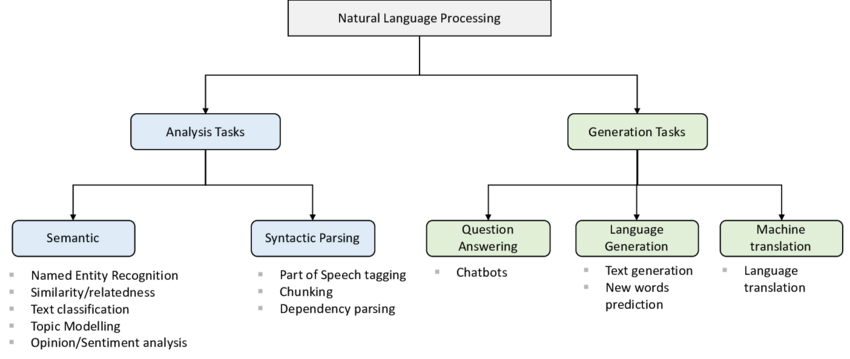
\includegraphics[width=0.5\textwidth]{assets/nlp/taxonomy.png}
    \caption{Таксономия современных подходов обработки естественного языка}
    \label{llm_taxonomy}
\end{figure}